
%% bare_conf_compsoc.tex
%% V1.4b
%% 2015/08/26
%% by Michael Shell
%% See:
%% http://www.michaelshell.org/
%% for current contact information.
%%
%% This is a skeleton file demonstrating the use of IEEEtran.cls
%% (requires IEEEtran.cls version 1.8b or later) with an IEEE Computer
%% Society conference paper.
%%
%% Support sites:
%% http://www.michaelshell.org/tex/ieeetran/
%% http://www.ctan.org/pkg/ieeetran
%% and
%% http://www.ieee.org/

%%*************************************************************************
%% Legal Notice:
%% This code is offered as-is without any warranty either expressed or
%% implied; without even the implied warranty of MERCHANTABILITY or
%% FITNESS FOR A PARTICULAR PURPOSE! 
%% User assumes all risk.
%% In no event shall the IEEE or any contributor to this code be liable for
%% any damages or losses, including, but not limited to, incidental,
%% consequential, or any other damages, resulting from the use or misuse
%% of any information contained here.
%%
%% All comments are the opinions of their respective authors and are not
%% necessarily endorsed by the IEEE.
%%
%% This work is distributed under the LaTeX Project Public License (LPPL)
%% ( http://www.latex-project.org/ ) version 1.3, and may be freely used,
%% distributed and modified. A copy of the LPPL, version 1.3, is included
%% in the base LaTeX documentation of all distributions of LaTeX released
%% 2003/12/01 or later.
%% Retain all contribution notices and credits.
%% ** Modified files should be clearly indicated as such, including  **
%% ** renaming them and changing author support contact information. **
%%*************************************************************************


% *** Authors should verify (and, if needed, correct) their LaTeX system  ***
% *** with the testflow diagnostic prior to trusting their LaTeX platform ***
% *** with production work. The IEEE's font choices and paper sizes can   ***
% *** trigger bugs that do not appear when using other class files.       ***                          ***
% The testflow support page is at:
% http://www.michaelshell.org/tex/testflow/

\documentclass[10pt, conference, compsocconf]{IEEEtran}
% Some/most Computer Society conferences require the compsoc mode option,
% but others may want the standard conference format.
%
% If IEEEtran.cls has not been installed into the LaTeX system files,
% manually specify the path to it like:
% \documentclass[conference,compsoc]{../sty/IEEEtran}

\usepackage{hyperref}

% PDF Settings
\hypersetup{
%    bookmarks=true,         % show bookmarks bar?
%    unicode=false,          % non-Latin characters in Acrobat�s bookmarks
%    pdftoolbar=true,        % show Acrobat's toolbar?
%    pdfmenubar=true,        % show Acrobat's menu?
%    pdffitwindow=false,     % window fit to page when opened
%    pdfstartview={FitH},    % fits the width of the page to the window
    pdftitle={Architecture and Design of Cray DataWarp},    % title
    pdfauthor={Dave Henseler, Benjamin Landsteiner, Doug Petesch, Cornell Wright, Nicholas J. Wright},     % author
    pdfsubject={DataWarp},   % subject of the document
%    pdfcreator={Creator},   % creator of the document
%    pdfproducer={Producer}, % producer of the document
    pdfkeywords={SSD, DataWarp, Architecture, Design, Filesystems}, % list of keywords
%    pdfnewwindow=true,      % links in new window
%    colorlinks=false,       % false: boxed links; true: colored links
%    linkcolor=red,          % color of internal links
%    citecolor=green,        % color of links to bibliography
%    filecolor=magenta,      % color of file links
%    urlcolor=cyan           % color of external links
}


% Some very useful LaTeX packages include:
% (uncomment the ones you want to load)


% *** MISC UTILITY PACKAGES ***
%
%\usepackage{ifpdf}
% Heiko Oberdiek's ifpdf.sty is very useful if you need conditional
% compilation based on whether the output is pdf or dvi.
% usage:
% \ifpdf
%   % pdf code
% \else
%   % dvi code
% \fi
% The latest version of ifpdf.sty can be obtained from:
% http://www.ctan.org/pkg/ifpdf
% Also, note that IEEEtran.cls V1.7 and later provides a builtin
% \ifCLASSINFOpdf conditional that works the same way.
% When switching from latex to pdflatex and vice-versa, the compiler may
% have to be run twice to clear warning/error messages.



% *** CITATION PACKAGES ***
%
\ifCLASSOPTIONcompsoc
  % IEEE Computer Society needs nocompress option
  % requires cite.sty v4.0 or later (November 2003)
  \usepackage[nocompress]{cite}
\else
  % normal IEEE
  \usepackage{cite}
\fi
% cite.sty was written by Donald Arseneau
% V1.6 and later of IEEEtran pre-defines the format of the cite.sty package
% \cite{} output to follow that of the IEEE. Loading the cite package will
% result in citation numbers being automatically sorted and properly
% "compressed/ranged". e.g., [1], [9], [2], [7], [5], [6] without using
% cite.sty will become [1], [2], [5]--[7], [9] using cite.sty. cite.sty's
% \cite will automatically add leading space, if needed. Use cite.sty's
% noadjust option (cite.sty V3.8 and later) if you want to turn this off
% such as if a citation ever needs to be enclosed in parenthesis.
% cite.sty is already installed on most LaTeX systems. Be sure and use
% version 5.0 (2009-03-20) and later if using hyperref.sty.
% The latest version can be obtained at:
% http://www.ctan.org/pkg/cite
% The documentation is contained in the cite.sty file itself.
%
% Note that some packages require special options to format as the Computer
% Society requires. In particular, Computer Society  papers do not use
% compressed citation ranges as is done in typical IEEE papers
% (e.g., [1]-[4]). Instead, they list every citation separately in order
% (e.g., [1], [2], [3], [4]). To get the latter we need to load the cite
% package with the nocompress option which is supported by cite.sty v4.0
% and later.





% *** GRAPHICS RELATED PACKAGES ***
%
\ifCLASSINFOpdf
  \usepackage[pdftex]{graphicx}
  % declare the path(s) where your graphic files are
  % \graphicspath{{../pdf/}{../jpeg/}}
  % and their extensions so you won't have to specify these with
  % every instance of \includegraphics
  % \DeclareGraphicsExtensions{.pdf,.jpeg,.png}
\else
  % or other class option (dvipsone, dvipdf, if not using dvips). graphicx
  % will default to the driver specified in the system graphics.cfg if no
  % driver is specified.
  % \usepackage[dvips]{graphicx}
  % declare the path(s) where your graphic files are
  % \graphicspath{{../eps/}}
  % and their extensions so you won't have to specify these with
  % every instance of \includegraphics
  % \DeclareGraphicsExtensions{.eps}
\fi
% This has to be after graphicx???
\usepackage{pgfplots}
\pgfplotsset{compat=1.13}
\usepgfplotslibrary{external}
\tikzexternalize

% graphicx was written by David Carlisle and Sebastian Rahtz. It is
% required if you want graphics, photos, etc. graphicx.sty is already
% installed on most LaTeX systems. The latest version and documentation
% can be obtained at: 
% http://www.ctan.org/pkg/graphicx
% Another good source of documentation is "Using Imported Graphics in
% LaTeX2e" by Keith Reckdahl which can be found at:
% http://www.ctan.org/pkg/epslatex
%
% latex, and pdflatex in dvi mode, support graphics in encapsulated
% postscript (.eps) format. pdflatex in pdf mode supports graphics
% in .pdf, .jpeg, .png and .mps (metapost) formats. Users should ensure
% that all non-photo figures use a vector format (.eps, .pdf, .mps) and
% not a bitmapped formats (.jpeg, .png). The IEEE frowns on bitmapped formats
% which can result in "jaggedy"/blurry rendering of lines and letters as
% well as large increases in file sizes.
%
% You can find documentation about the pdfTeX application at:
% http://www.tug.org/applications/pdftex





% *** MATH PACKAGES ***
%
%\usepackage{amsmath}
% A popular package from the American Mathematical Society that provides
% many useful and powerful commands for dealing with mathematics.
%
% Note that the amsmath package sets \interdisplaylinepenalty to 10000
% thus preventing page breaks from occurring within multiline equations. Use:
%\interdisplaylinepenalty=2500
% after loading amsmath to restore such page breaks as IEEEtran.cls normally
% does. amsmath.sty is already installed on most LaTeX systems. The latest
% version and documentation can be obtained at:
% http://www.ctan.org/pkg/amsmath





% *** SPECIALIZED LIST PACKAGES ***
%
%\usepackage{algorithmic}
% algorithmic.sty was written by Peter Williams and Rogerio Brito.
% This package provides an algorithmic environment fo describing algorithms.
% You can use the algorithmic environment in-text or within a figure
% environment to provide for a floating algorithm. Do NOT use the algorithm
% floating environment provided by algorithm.sty (by the same authors) or
% algorithm2e.sty (by Christophe Fiorio) as the IEEE does not use dedicated
% algorithm float types and packages that provide these will not provide
% correct IEEE style captions. The latest version and documentation of
% algorithmic.sty can be obtained at:
% http://www.ctan.org/pkg/algorithms
% Also of interest may be the (relatively newer and more customizable)
% algorithmicx.sty package by Szasz Janos:
% http://www.ctan.org/pkg/algorithmicx




% *** ALIGNMENT PACKAGES ***
%
%\usepackage{array}
% Frank Mittelbach's and David Carlisle's array.sty patches and improves
% the standard LaTeX2e array and tabular environments to provide better
% appearance and additional user controls. As the default LaTeX2e table
% generation code is lacking to the point of almost being broken with
% respect to the quality of the end results, all users are strongly
% advised to use an enhanced (at the very least that provided by array.sty)
% set of table tools. array.sty is already installed on most systems. The
% latest version and documentation can be obtained at:
% http://www.ctan.org/pkg/array


% IEEEtran contains the IEEEeqnarray family of commands that can be used to
% generate multiline equations as well as matrices, tables, etc., of high
% quality.




% *** SUBFIGURE PACKAGES ***
\ifCLASSOPTIONcompsoc
  \usepackage[caption=false,font=footnotesize,labelfont=sf,textfont=sf]{subfig}
\else
  \usepackage[caption=false,font=footnotesize]{subfig}
\fi
% subfig.sty, written by Steven Douglas Cochran, is the modern replacement
% for subfigure.sty, the latter of which is no longer maintained and is
% incompatible with some LaTeX packages including fixltx2e. However,
% subfig.sty requires and automatically loads Axel Sommerfeldt's caption.sty
% which will override IEEEtran.cls' handling of captions and this will result
% in non-IEEE style figure/table captions. To prevent this problem, be sure
% and invoke subfig.sty's "caption=false" package option (available since
% subfig.sty version 1.3, 2005/06/28) as this is will preserve IEEEtran.cls
% handling of captions.
% Note that the Computer Society format requires a sans serif font rather
% than the serif font used in traditional IEEE formatting and thus the need
% to invoke different subfig.sty package options depending on whether
% compsoc mode has been enabled.
%
% The latest version and documentation of subfig.sty can be obtained at:
% http://www.ctan.org/pkg/subfig




% *** FLOAT PACKAGES ***
%
%\usepackage{fixltx2e}
% fixltx2e, the successor to the earlier fix2col.sty, was written by
% Frank Mittelbach and David Carlisle. This package corrects a few problems
% in the LaTeX2e kernel, the most notable of which is that in current
% LaTeX2e releases, the ordering of single and double column floats is not
% guaranteed to be preserved. Thus, an unpatched LaTeX2e can allow a
% single column figure to be placed prior to an earlier double column
% figure.
% Be aware that LaTeX2e kernels dated 2015 and later have fixltx2e.sty's
% corrections already built into the system in which case a warning will
% be issued if an attempt is made to load fixltx2e.sty as it is no longer
% needed.
% The latest version and documentation can be found at:
% http://www.ctan.org/pkg/fixltx2e


\usepackage{stfloats}
% stfloats.sty was written by Sigitas Tolusis. This package gives LaTeX2e
% the ability to do double column floats at the bottom of the page as well
% as the top. (e.g., "\begin{figure*}[!b]" is not normally possible in
% LaTeX2e). It also provides a command:
%\fnbelowfloat
% to enable the placement of footnotes below bottom floats (the standard
% LaTeX2e kernel puts them above bottom floats). This is an invasive package
% which rewrites many portions of the LaTeX2e float routines. It may not work
% with other packages that modify the LaTeX2e float routines. The latest
% version and documentation can be obtained at:
% http://www.ctan.org/pkg/stfloats
% Do not use the stfloats baselinefloat ability as the IEEE does not allow
% \baselineskip to stretch. Authors submitting work to the IEEE should note
% that the IEEE rarely uses double column equations and that authors should try
% to avoid such use. Do not be tempted to use the cuted.sty or midfloat.sty
% packages (also by Sigitas Tolusis) as the IEEE does not format its papers in
% such ways.
% Do not attempt to use stfloats with fixltx2e as they are incompatible.
% Instead, use Morten Hogholm'a dblfloatfix which combines the features
% of both fixltx2e and stfloats:
%
% \usepackage{dblfloatfix}
% The latest version can be found at:
% http://www.ctan.org/pkg/dblfloatfix




% *** PDF, URL AND HYPERLINK PACKAGES ***
%
\usepackage{url}
% url.sty was written by Donald Arseneau. It provides better support for
% handling and breaking URLs. url.sty is already installed on most LaTeX
% systems. The latest version and documentation can be obtained at:
% http://www.ctan.org/pkg/url
% Basically, \url{my_url_here}.




% *** Do not adjust lengths that control margins, column widths, etc. ***
% *** Do not use packages that alter fonts (such as pslatex).         ***
% There should be no need to do such things with IEEEtran.cls V1.6 and later.
% (Unless specifically asked to do so by the journal or conference you plan
% to submit to, of course. )


% correct bad hyphenation here
\hyphenation{Data-Warp}


\begin{document}
%
% paper title
% Titles are generally capitalized except for words such as a, an, and, as,
% at, but, by, for, in, nor, of, on, or, the, to and up, which are usually
% not capitalized unless they are the first or last word of the title.
% Linebreaks \\ can be used within to get better formatting as desired.
% Do not put math or special symbols in the title.
\title{Architecture and Design of Cray DataWarp}


% author names and affiliations
% use a multiple column layout for up to three different
% affiliations
%\author{\IEEEauthorblockN{Michael Shell}
%\IEEEauthorblockA{School of Electrical and\\Computer Engineering\\
%Georgia Institute of Technology\\
%Atlanta, Georgia 30332--0250\\
%Email: http://www.michaelshell.org/contact.html}
%\and
%\IEEEauthorblockN{Homer Simpson}
%\IEEEauthorblockA{Twentieth Century Fox\\
%Springfield, USA\\
%Email: homer@thesimpsons.com}
%\and
%\IEEEauthorblockN{James Kirk\\ and Montgomery Scott}
%\IEEEauthorblockA{Starfleet Academy\\
%San Francisco, California 96678-2391\\
%Telephone: (800) 555--1212\\
%Fax: (888) 555--1212}}

% conference papers do not typically use \thanks and this command
% is locked out in conference mode. If really needed, such as for
% the acknowledgment of grants, issue a \IEEEoverridecommandlockouts
% after \documentclass

% for over three affiliations, or if they all won't fit within the width
% of the page (and note that there is less available width in this regard for
% compsoc conferences compared to traditional conferences), use this
% alternative format:
% 
\author{\IEEEauthorblockN{Dave Henseler\IEEEauthorrefmark{1},
Benjamin Landsteiner\IEEEauthorrefmark{1},
Doug Petesch\IEEEauthorrefmark{1},
Cornell Wright\IEEEauthorrefmark{2}, and
Nicholas J. Wright\IEEEauthorrefmark{3}}
\IEEEauthorblockA{\IEEEauthorrefmark{1}Cray Inc., Saint Paul, MN  55101\\
Email: \{dah, ben, dpetesch\}@cray.com}
\IEEEauthorblockA{\IEEEauthorrefmark{2}Los Alamos National Laboratory, Los Alamos, NM  87544\\
Email: cornell@lanl.gov}
\IEEEauthorblockA{\IEEEauthorrefmark{3}Lawrence Berkeley National Laboratory\\
National Energy Research Scientific Computing Center, Berkeley, CA  94720\\
Email: njwright@lbl.gov}}




% use for special paper notices
%\IEEEspecialpapernotice{(Invited Paper)}




% make the title area
\maketitle

% As a general rule, do not put math, special symbols or citations
% in the abstract
\begin{abstract}
This paper describes the architecture, design, use, and performance of Cray DataWarp.  DataWarp is an infrastructure that uses direct-attached solid-state disk~(SSD) storage to provide more cost-effective bandwidth than an external parallel file system~(PFS), allowing DataWarp to be provisioned for bandwidth and the PFS to be provisioned for capacity and resiliency. Placing this storage between the application and the PFS allows application I/O to be decoupled from PFS I/O and in some cases avoiding it altogether. This reduces the time required for the application to do I/O, while also increasing the overlap of computation with PFS I/O, typically reducing application elapsed time. DataWarp allocates and configures SSD-backed storage for jobs and users on demand, providing many of the benefits of both software defined storage and storage virtualization.
\end{abstract}

\begin{IEEEkeywords}
Filesystems \& I/O, DataWarp, SSD
\end{IEEEkeywords}



% For peer review papers, you can put extra information on the cover
% page as needed:
% \ifCLASSOPTIONpeerreview
% \begin{center} \bfseries EDICS Category: 3-BBND \end{center}
% \fi
%
% For peerreview papers, this IEEEtran command inserts a page break and
% creates the second title. It will be ignored for other modes.
\IEEEpeerreviewmaketitle



\section{Introduction}
Although hard disk drive~(HDD) capacity has increased significantly in recent years, HDD bandwidth increases have been much more modest. In contrast, solid-state disk~(SSD) devices provide high bandwidth and their prices have been declining. At the present time, SSD bandwidth~(\$~/~GB~/~second) is less expensive than HDD bandwidth. This leads to SSDs being the economically preferable device for use cases dominated by bandwidth considerations.  Placing SSD storage between the application and a HDD-backed Parallel File System~(PFS) such as Lustre~\cite{lustre_manual} or GPFS~\cite{gpfs_manual} can allow the PFS to be more cost-effective as it only needs to be provisioned for capacity and resiliency rather than peak bandwidth. This also reduces the cost of connectivity from the supercomputer to the PFS. Placing this storage between the application and the PFS allows application I/O to be decoupled from PFS I/O and in some cases avoiding it altogether.  This reduces the time required for the application to do I/O, increases the overlap of computation with PFS I/O, and typically reduces application elapsed time.

Cray DataWarp software allocates and configures SSD-backed storage for jobs and users, providing many of the benefits of both software-defined storage~\cite{sds-snia} and storage virtualization.  This includes automation, standard APIs, virtualized data path, scalability, and transparency.  DataWarp is an implementation of the burst buffer concept~\cite{6232369} for Cray systems, and more.

Automated tasks include on-demand allocation, configuration, and migration of data to and from a PFS.  Users request use of DataWarp primarily through simple job script directives and then use DataWarp through POSIX APIs.  If desired, a C library provides an additional way for applications to make use of DataWarp.  Command line tools expose functionality in a RESTful interface that is capable of showing status and requesting a particular configuration.  DataWarp configures compute nodes to interact with their assigned storage and provides for per-instance metadata.  Striping across multiple server nodes allows DataWarp to have access to additional capacity and bandwidth.  Use of DataWarp is optional and job script directives specify the degree to which data is intended to be exposed and shared to other jobs.  Workload Managers~(WLMs) manage the lifetime of storage allocations to jobs and ensure that requested capacity remains dedicated to jobs for as long as is needed.  

PCI-attached SSDs are located on Cray XC service nodes connected directly to the Aries high speed network. The SSD bandwidth is closely matched to the Aries bandwidth, taking maximum advantage of the Aries network and avoiding the additional cost of provisioning connectivity and bandwidth to external SSDs.

%Although hard disk drive (HDD) capacity has increased significantly in recent years, HDD bandwidth increases have been much more modest. In contrast, SSD devices provide high bandwidth and their prices have been declining. At the present time, SSD bandwidth (\$~/~GB~/~second) is less expensive than HDD bandwidth. This leads to SSDs being the economically preferable device for use cases dominated by bandwidth considerations, and it can allow the PFS to be more cost-effective as it only needs to be provisioned for capacity and resiliency rather than peak bandwidth. This also reduces the cost of connectivity from the supercomputer to the PFS. Placing this storage between the application and the PFS allows application I/O to be decoupled from (or in some cases eliminating) PFS I/O.  This reduces the time required for the application to do I/O, increases the overlap of computation with PFS I/O, and typically reduces application elapsed time.

DataWarp will be released in four phases.  Each phase introduces new features and refines or replaces the functionality present in prior phases.
\subsection{Phase~0}
Phase~0 supports statically configured compute node swap and single server scratch file systems.  Cray released Phase~0 in CLE5.2.UP02 in Fall 2014.
\subsection{Phase~1}
Phase~1 supports dynamic allocation and configuration of DataWarp storage to jobs.  This includes requests for swap, and job- and application-controlled explicit data movement between DataWarp and PFS storage.  An instance of storage that supports explicitly moving data is described hereafter as a \emph{scratch instance}.  Applications interact with scratch instances through mount points and explicitly request data to be copied between the scratch instance and PFS via job script-accessible and application-accessible APIs.  Scratch instances also support policies intended to detect and halt excess I/O activity that would otherwise lead to premature SSD failure.  Phase~1 supersedes Phase~0, though DataWarp server nodes can still be used with the Phase~0 infrastructure by isolating them from the Phase~1 configuration.  Cray released Phase~1 in CLE5.2.UP04 in Fall 2015.
\subsection{Phase~2}
Phase~2 adds implicit movement of data between DataWarp and PFS storage, described hereafter as a \emph{cached instance}.  It also includes accounting support and Data Virtualization Service~(DVS)~\cite{dvs_admin} client-side caching.  With a cached instance, job scripts and applications are only required to switch from using a PFS mount point to using a DataWarp mount point.  When using the DataWarp mount point, I/O between the application and PFS is transparently buffered on the DataWarp server nodes.  Jobs and applications may additionally interact with the cached instance through other APIs to further improve performance.  Cached instances support excess I/O activity detection as in Phase~1.  The accounting functionality works with scratch and cached instances and measures I/O interactions  between compute nodes and DataWarp nodes.  DVS client-side caching improves performance for workloads with small reads and writes.  Cray plans to release Phase~2 in Summer 2016.
\subsection{Phase~3}
Phase~3 adds the ability to run applications directly on DataWarp server nodes.  It also includes improved resiliency and recovery support, and allows jobs to request multiple job instances per job.  Cray plans to release Phase~3 in Winter 2016.

\section{Use Cases}
The following is a list of anticipated use cases that will leverage the functionality of DataWarp.

\subsection{Parallel File System Cache}
DataWarp can be used to cache PFS data. Unlike SSD caching infrastructures that provide a block-based cache between a file system and a hard disk, DataWarp provides a file-based cache between the application and a PFS. The DataWarp server software is fully integrated with both the kernel page cache and the PFS client.

Some examples of PFS cache use cases are:
\begin{itemize}
\item \textbf{Checkpoint/Restart:} In order to tolerate both compute node and system failures, applications can periodically write checkpoint files. All checkpoints are first written to DataWarp to take advantage of the high bandwidth. Some of those checkpoints reside only on DataWarp and support fast restart in the event of a compute node failure. Other checkpoints will be asynchronously copied by DataWarp to the PFS to support restart in the event of a system failure.  Job script directives and C library functions allow users to specify the policy behind which files are copied to the PFS and when.
\item \textbf{Periodic output:} Applications that produce periodic output (for example time series data) can write those results to DataWarp and then resume computation while DataWarp copies that data to the PFS asynchronously.
\item \textbf{Application libraries:} Some applications reference a large number of libraries from every rank, for example Python-based applications. Those libraries can be copied from the PFS to DataWarp once and used by all ranks directly from DataWarp storage.
\end{itemize}
When using a DataWarp scratch instance, movement of data between DataWarp and the PFS is explicitly requested by the job and/or the application and is performed by the DataWarp service. When using a DataWarp cached instance, movement of data between DataWarp and the PFS can also be done implicitly (read ahead and write behind) by the DataWarp service without any intervention from the application.

\subsection{Application Scratch}
DataWarp can provide storage that functions like a big \verb+/tmp+ file system for each compute node in a job. Applications that use ``out-of-core'' algorithms could use DataWarp storage this way. Typically this data never reaches the PFS, but it can if desired by using job script directives or C library functions.

\subsection{Shared Data}
DataWarp can provide storage for data that is shared by multiple jobs over long periods of time. The jobs may be related or not, and may run concurrently or serially. Use cases include:
\begin{itemize}
\item \textbf{Shared input:} This would usually be a read-only input file or database, for example a bioinformatics database used as input by multiple analysis jobs. The data can be copied from PFS to DataWarp once and then shared by many jobs.
\item \textbf{Ensemble analysis:} This is often a special case of the shared input case for a set of similar runs with different parameters on the same inputs, but could also allow for some minor modification of the input data across the runs in a set. Many simulation strategies make use of ensembles.
\item \textbf{In-transit analysis:} This refers to passing the results of one job to the input of a subsequent job, typically using WLM job dependencies. The data can reside only on DataWarp storage and never touch the PFS. This includes various types of workflows that go through a sequence of processing steps, transforming the input data along the way for each step. This can also be used for processing of intermediate results while an application is running, for example visualization or analysis of partial results, potentially even for steering the main application.
\end{itemize}

\subsection{Compute Node Swap}
DataWarp can provide compute node swap for jobs that require it. This is often needed by pre- and post-processing jobs that cannot fit in compute node memory and therefore need to swap during execution.  If only unused system libraries and services are swapped out (i.e., the application only needs a small amount of additional compute node memory) the performance penalty to the application is limited to the initial swap out and application performance may improve.

As with any swap implementation, swap performance is only acceptable for limited or transient overcommitments of node memory. For swap to SSD, excessive swapping can reduce the SSD endurance disproportionate to other uses.

\subsection{Applications Running On DataWarp Server Nodes}
DataWarp can allow applications to run directly on DataWarp server nodes, giving the applications direct access to the local performance of the SSD storage.  Specifically, the high input/output operations per second~(IOPS) rate for small transfers, file creation, and file deletion.  This will place specific ranks/PEs on the DataWarp server nodes running in the same MPI\_COMM\_WORLD communicator as ranks on compute nodes.

The DataWarp server nodes used to host applications are dedicated for this purpose only. They are treated as compute nodes, requested explicitly by a job and allocated exclusively to a job by the WLM. Administrators can manually move DataWarp server nodes between this use and normal DataWarp use.

\section{Architecture, Design, and Implementation}
This section describes the architecture, design, and implementation of DataWarp.  See \figurename~\ref{hwarch} for a pictorial representation of the hardware architecture.  Compute nodes~(CN) access DataWarp~(DW) over the high-speed Aries network.  DataWarp nodes access PFS resources, such as Lustre, via a path that traverses both the Aries network and non-Aries network, such as Infiniband.  

\figurename~\ref{arch_comp} shows the software architecture component diagram.  WLMs work with DataWarp to ensure compute node applications have access to DataWarp resources.  Files can be staged between DataWarp and a PFS via job script requests or application requests routed to DataWarp through DVS.  Application I/O is routed to DataWarp servers through DVS.  Application data is temporarily stored on DataWarp server SSDs in order to accelerate application I/O operations.

\begin{figure*}
\centering
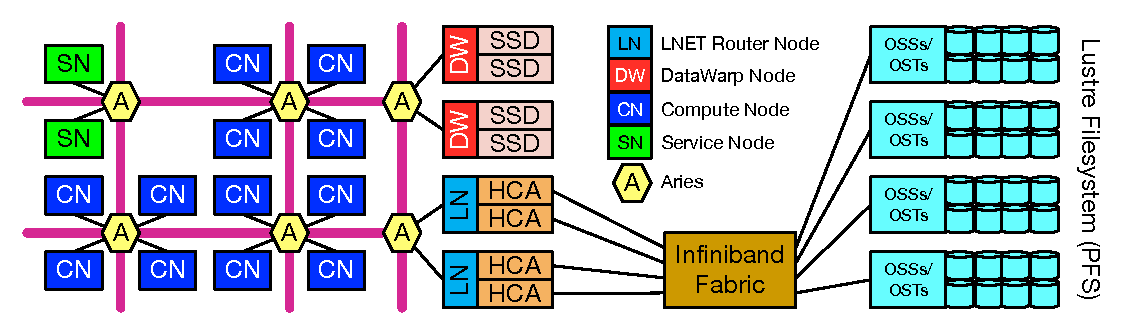
\includegraphics[width=\textwidth]{graphics/hwarch}
\caption{DataWarp hardware architecture overview.\label{hwarch}}
\end{figure*}
\begin{figure*}
\centering
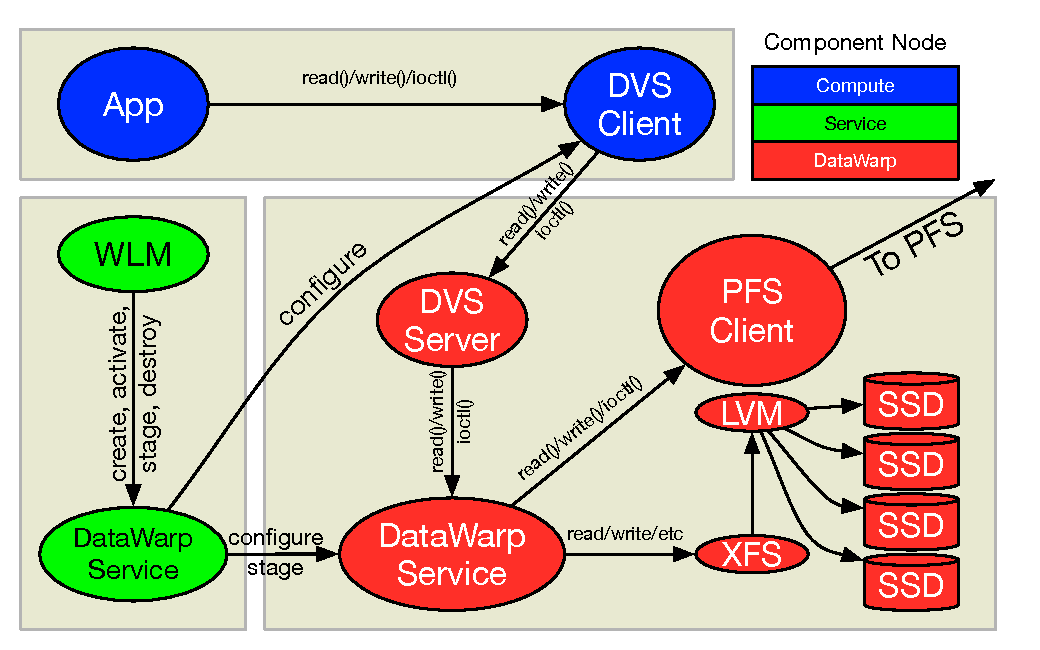
\includegraphics[width=0.8\textwidth]{graphics/arch_comp}
\caption{DataWarp software architecture component diagram.\label{arch_comp}}
\end{figure*}

\subsection{Instances}
When requested, DataWarp storage space is assigned dynamically and in the amount requested.  This is referred to as an \emph{instance}. The space is allocated on one or more DataWarp server nodes and is dedicated to the instance for its lifetime.  The space taken on each node for the instance is referred to as a \emph{fragment}. The requested capacity is used as a job scheduling constraint by the WLM.

The bandwidth associated with an instance is dedicated to it if there is only one instance present on the assigned DataWarp server nodes. For example, if two jobs each request half the total DataWarp capacity and each job gets exclusive access to all the capacity on half the DataWarp server nodes, then each job gets half the total DataWarp bandwidth. Conversely, if each job gets half the capacity on all DataWarp server nodes, each job gets all of the total DataWarp bandwidth when their I/O does not overlap.  In the first example, performance is more deterministic, but depending on the degree of I/O overlap, the second example application's I/O may perform up to twice as fast.

A DataWarp instance has a lifetime that is specified when it is created and can be one of:
\begin{itemize}
\item \textbf{Job instance:} A \emph{job instance} lifetime is the same as the lifetime of the job that created it (created at job start, destroyed at job end), and is accessible only by the compute nodes allocated to the job that created it. A job instance is relevant to all use cases except shared data.
\item \textbf{Persistent instance:} A \emph{persistent instance} lifetime is not tied to the lifetime of any single job. Access can be requested by any job, but file access is authenticated and authorized based on the POSIX file permissions of the individual files and directories. Jobs request access to a persistent instance by providing the persistent instance's name in a job script directive. A persistent instance is relevant to the shared data use case. Persistent instances are explicitly created by a user, typically outside of a job, since their lifetime is not associated with any job's lifetime.
\end{itemize}
When an instance is destroyed, DataWarp will ensure that any data that needs to be written to the PFS has been before it releases the space for reuse. In the case of a job instance, this can delay the completion of the job.

\subsection{Application I/O}
The DataWarp service dynamically configures access to DataWarp instances on all compute nodes assigned to a job using a given instance. Application I/O is forwarded from compute nodes to the instance's DataWarp server nodes using the Data Virtualization Service~(DVS).  DVS provides POSIX-based file system access to the DataWarp storage.

A DataWarp instance can be configured as one of three types:
\begin{itemize}
\item \textbf{Scratch:} When using a scratch instance (i.e., DataWarp Phase~1) all movement of data between the instance and the PFS must be explicitly requested using the DataWarp API. The actual data transfers are performed directly between the DataWarp nodes and the PFS.
\item \textbf{Cached:} When using a cached instance (i.e., DataWarp Phase~2) all movement of data between the instance and the PFS is done implicitly. The instance configuration and application-accessible C API can change the implicit behavior.
\item \textbf{Swap:} When using a swap instance, swap files are created on a DataWarp instance that compute nodes access over iSCSI. 
\end{itemize}

An instance can be scratch, cached, swap, scratch+swap, or cached+swap, but never scratch+cached.  A single instance used for scratch+cached would lead to scratch usages of the instance running out of space, as the cached usage would fill up the instance in order to maximize cache hits.  Phase~3 will allow for jobs to request multiple job instances which will allow for a job to request both a scratch and a cached instance.

A scratch or cached instance can be accessed in one or more of the following ways:
\begin{itemize}
\item \textbf{Striped:} In striped access mode, individual files are striped across multiple DataWarp server nodes (aggregating both capacity and bandwidth per file) and are accessible by all compute nodes using the instance.
\item \textbf{Private:} In private access mode, individual files are striped across multiple DataWarp server nodes (aggregating both capacity and bandwidth per file) but the files are only accessible to the compute node that created them (e.g. like \verb+/tmp+). Private access is not supported for persistent instances because a persistent instance can be used by multiple jobs with different numbers of compute nodes; it is not supported for cached instances because all files are visible in the PFS.
\item \textbf{Load-balanced:} In load-balanced access mode, individual files are replicated (read-only) on multiple DataWarp server nodes (aggregating bandwidth but not capacity per instance), and compute nodes choose one of the replicas to use. Load-balanced mode is useful when the files are not large enough to stripe across a sufficient number of nodes.
\end{itemize}

Each permutation of instance (job or persistent), type (scratch or cached), and access mode (striped, private, or load-balanced) maps to unique mount points on the compute nodes. The mount point for each is provided to the job via environment variables.  See Table~\ref{am_support} for the valid combinations of access mode, configuration, and instance type.



\begin{table}[htbp]
\renewcommand{\arraystretch}{1.3}
\caption{Access mode support for scratch and cached configurations\label{am_support}}
\centering
\begin{tabular}{r|cc|cc}
\multicolumn{1}{c}{}&\multicolumn{2}{c|}{Job Instance}&\multicolumn{2}{c}{Persistent Instance}\\
\hline
access mode&scratch&cached&scratch&cached\\
\hline
striped&yes&yes&yes&yes\\
private&yes&no&no&no\\
load-balanced&yes&yes&yes&yes\\
\end{tabular}
\end{table}

Within a scratch instance, the directory structure (and associated directory overhead) for the instance is managed differently depending on the access mode: for striped access, one of the DataWarp servers manages the directory for the instance; for private and load-balanced access, each DataWarp server manages the directories for files assigned to it. Within a cached instance, the directory structure resides on the PFS itself, and every DataWarp server can access it directly.

Every DataWarp server performs PFS I/O for the files and stripes that reside on it. This provides parallel access to the PFS, but from fewer nodes than if it had been directly accessed from compute nodes. For a scratch instance, PFS I/O is explicitly initiated by the job or application, and it transfers an entire file to or from the DataWarp server nodes. For a cached instance, PFS I/O is implicitly initiated by the DataWarp service based on modified data thresholds, the DataWarp file system becoming full, or reads of data not currently present. The DataWarp service manages space using least-recently-used tracking and provides read-ahead and write-behind functionality.  As a result, the file system never becomes full since it is always able to flush modified data to, or to reclaim data from, the PFS.

\subsection{Workload Manager Integration}
Multiple workload managers~(WLMs), including Moab/TORQUE~\cite{moab_admin,torque_admin}, PBS~\cite{pbs_admin}, and Slurm~\cite{slurm_docs}, support DataWarp on Cray systems.  DataWarp directives are specified in the job script file and passed to the DataWarp infrastructure by the WLM at various points in a job lifetime. These callouts allow DataWarp to:
\begin{itemize}
\item Create/configure instances on DataWarp server nodes
\item Stage files between a PFS and DataWarp instances (without compute nodes assigned if the WLM supports it), at both the beginning and end of a job
\item Configure/unconfigure compute node access to DataWarp instances
\item Unconfigure/clean-up instances on DataWarp server nodes
\end{itemize}

The DataWarp job script directives include the ability to:
\begin{itemize}
\item Create and configure compute node access to a DataWarp job scratch instance:\\
{\footnotesize \texttt{\#DW jobdw type=scratch access\_mode=[striped,private,loadbalance] capacity=n \ldots}}
\item Create and configure compute node access to a DataWarp job cached instance:\\
{\footnotesize \texttt{\#DW jobdw type=cache access\_mode=[striped,loadbalance] capacity=n pfs=path \ldots}}
\item Configure compute node access to a DataWarp persistent instance:\\
{\footnotesize \texttt{\#DW persistentdw name=xxx}}
\item Create swap space for each compute node in a job:\\
{\footnotesize \texttt{\#DW swap nGiB}}
\item Stage files from the PFS to DataWarp storage before a job runs:\\
{\footnotesize \texttt{\#DW stage\_in type=file\textbar{}directory\textbar{}list source=path destination=path}}
\item Stage files from DataWarp storage to the PFS after a job completes:\\
{\footnotesize \texttt{\#DW stage\_out type=file\textbar{}directory\textbar{}list source=path destination=path}}
\end{itemize}
The \texttt{\#DW jobdw} directive takes many additional optional parameters that allow users to specify I/O limits and set additional type-specific attributes.  For detail refer to the DataWarp User Guide~\cite{dw_user_guide}.

The capacity requested for a DataWarp instance is a consumable resource, used by the WLM as a scheduling constraint.  This means that jobs requesting DataWarp capacity will only start execution when that capacity is available and can be dedicated to the job.

If the WLM supports it, stage-in may be done before compute resources are assigned to the job and stage-out after those compute resources have been released.  This enhancement can significantly decrease the amount of time compute nodes are assigned; see \figurename~\ref{minimize_computes}.


\begin{figure*}
\centering
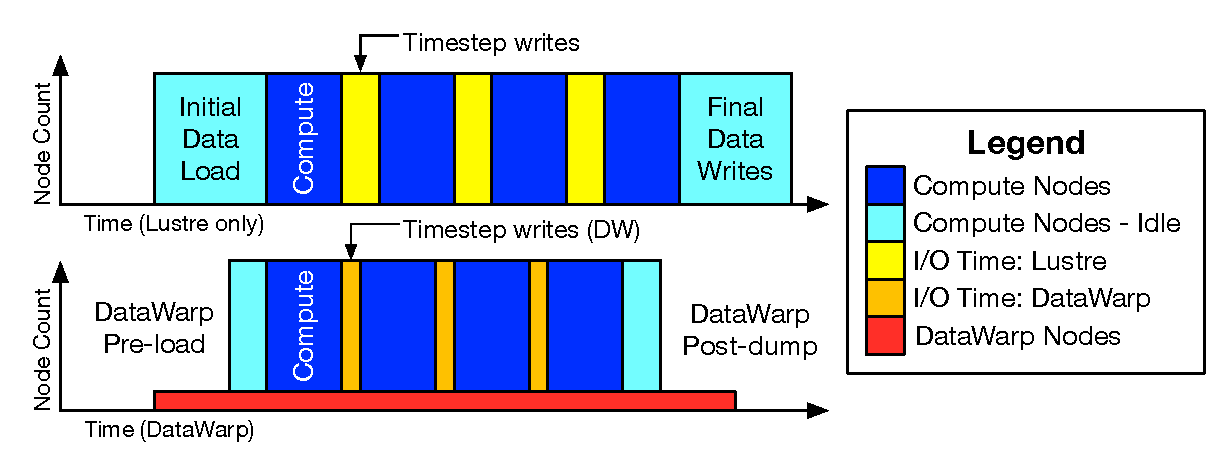
\includegraphics[width=\textwidth]{graphics/minimize_computes}
\caption{Loading up and draining DataWarp before compute nodes are assigned can reduce the amount of time compute nodes are allocated to a job and idling.  I/O performed during an application's lifetime is also accelerated if interacting with DataWarp since DataWarp bandwidth exceeds PFS bandwidth. \label{minimize_computes}}
\end{figure*}

\subsection{Job Example}
See \figurename~\ref{job_example} for an example of a job that requests a 100TiB capacity DataWarp job instance, references an existing DataWarp persistent instance, requests staging-in of a file, and requests staging-out a directory.

\begin{figure*}
\small
\begin{verbatim}
#!/bin/sh
#DW jobdw type=scratch access_mode=striped,private capacity=100TiB
#DW persistentdw name=rrr
#DW stage_in type=file source=/pfs/user/input destination=$DW_JOB_STRIPED/input
#DW stage_out type=directory source=$DW_JOB_STRIPED/results/ destination=/pfs/user/results/

export TMPDIR=$DW_JOB_PRIVATE
aprun -n 5000 a.out --tmpfiles=$DW_JOB_PRIVATE \
    --database=$DW_PERSISTENT_STRIPED_rrr/abc \
    --parameter-file=$DW_JOB_STRIPED/input \
    --resultsdir=$DW_JOB_STRIPED/results
\end{verbatim}
\caption{Example job script with DataWarp \#DW directives.  This batch job requests a 100TiB scratch instance with access modes striped and private.  It also requests access to the persistent DataWarp instance named rrr.  The user's parameter file input is staged into the job scratch instance before the aprun executes, and the result files are staged back out to the PFS after the aprun completes.\label{job_example}}
\end{figure*}

The DataWarp-enabled job file is submitted to the WLM just like any job file, e.g., for Slurm one would use \verb+sbatch job.sh+.  Each compute node has striped access to the persistent instance named \verb+rrr+ via the path defined by \verb+$DW_PERSISTENT_STRIPED_rrr+, striped access to the job instance via the path specified by \verb+$DW_JOB_STRIPED+, and private access via the path referenced at \verb+$DW_JOB_PRIVATE+.

\subsection{Application Programming Interfaces}
DataWarp provides command-line clients to query and control the DataWarp configuration. In addition to the job script directives discussed previously, there are commands to create and destroy persistent instances, list instances, list job references to instances, query server node state, and more. Some commands or their functionality are limited to administrators only.  In general, administrative users can see all DataWarp configuration and non-administrators can only see persistent instances and any configuration data associated with their userid.

All command-line clients interact with the DataWarp RESTful API over HTTPS.  All requests for DataWarp status, set up, job-directed staging, and teardown go through this API.  Users are authenticated with MUNGE~\cite{munge_install} and authorized in accordance with site configuration.

DataWarp also provides a C library API for use by applications which includes starting, querying, waiting, and terminating stage activity between a PFS and a DataWarp instance.  It also allows for retrieving or setting the stripe configuration of a file.  For cached instances, the library additionally supports getting and setting the modified threshold, read-ahead policy, and sync behavior policy.  Staging can be asynchronous with respect to an application or job, is performed concurrently from all DataWarp servers assigned to an instance, and can be done immediately or deferred until the end of a job.  A user might stage out only the last successful application-directed checkpoint-restart files.

In addition, some POSIX API calls have unique semantics when used with DataWarp:
\begin{itemize}
\item \textbf{statfs:} will return the aggregate size of the DataWarp instance, with the free space computed as the product of the number of servers and the current free capacity of the server with the least currently free space since that server will likely fill up first.
\item \textbf{stat:} stat information is only guaranteed to be accurate when a file is not open for write (i.e., it is updated at close).
\item \textbf{sync:} (only for type=cache) The behavior of a POSIX sync, fsync, or fdatasync call is controlled by the value of the sync\_to\_pfs attribute for a file, where the default is specified per instance. If true then it will sync data from DataWarp storage to the PFS. If false, a sync operation will just sync modified data cached in the DataWarp server's node memory to the DataWarp instance's storage file system.
\item \textbf{close:} (only for type=cache) The behavior of a POSIX close is controlled by the value of the sync\_on\_close for a file, where the default is specified per instance. If true then the close will sync data to the PFS. If false, close will just sync modified data cached in the DataWarp instance's server node memory to the DataWarp instance storage file system.
\item \textbf{unlink:} (only for type=cache) A POSIX unlink operation will remove the PFS file and remove all DataWarp instance state and data related to the file. If the file is open, the invalidate and removal is deferred until the last close.
\item \textbf{POSIX permissions:} (for type=cache and staging with type=scratch) The ability to access files (e.g. open, create, unlink, read, write, etc.) is controlled by the PFS permissions on directories and files.
\end{itemize}

\subsection{Storage Management}
A DataWarp server node contains one or more PCI SSD cards.  Architecturally, any block storage device could work but only qualified SSDs are supported. The Logical Volume Manager~(LVM) software~\cite{lvm} is used to aggregate the SSD cards on a server into a volume group and to partition the volume group into striped logical volumes on demand. When creating an instance, the DataWarp service configures the instance by creating logical volumes from the currently unallocated storage on as many server nodes as are needed to satisfy the requested capacity.  Depending on the site configuration and request preference, capacity can be chosen optimizing for bandwidth (use more servers) or minimal interference (use fewer servers).  Each piece of an instance on each server is called a \emph{fragment}.  See \figurename~\ref{3_inst} for an example with three instances and varying numbers of fragments spread across up to three servers.

\begin{figure*}
\centering
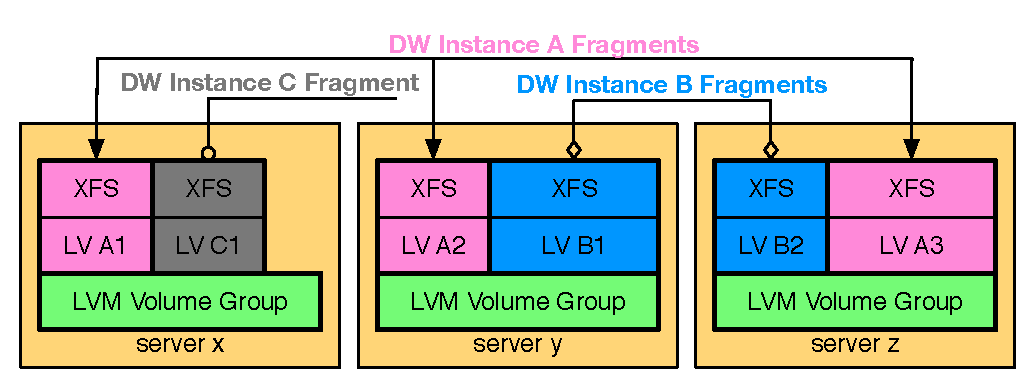
\includegraphics[width=0.8\textwidth]{graphics/3_inst}
\caption{Three DataWarp instances A, B, and C mapped to three servers, x, y, and z.  Instance A consists of fragments that map to LVM logical volumes A1, A2, and A3 on servers x, y, and z, respectively. Instance B consists of fragments that map to LVM logical volumes B1 and B2 on servers y and z, respectively. Instance C consists of a single fragment that maps to LVM logical volume C1 on server x.\label{3_inst}}
\end{figure*}

An XFS file system is created on each logical volume to manage the storage space~\cite{xfs_site}. XFS is a reliable and high performance file system for use with DataWarp.  It provides:
\begin{itemize}
\item integration with striped LVM volumes
\item SSD TRIM
\item configurable allocation sizes
\item scalable space allocation, file creation, and file deletion
\item extended attributes, and
\item space management APIs
\end{itemize}
The DVS stripe size is managed by the DataWarp service, taking into consideration the:
\begin{itemize}
\item SSD erasure block size to minimize write amplification
\item LVM stripe size to maximize device concurrency 
\item XFS allocation and stripe unit sizes, and
\item PFS stripe size to minimize lock conflicts on shared files
\end{itemize}

Each DataWarp server node on a system can be configured either for use by the DataWarp infrastructure (described in this paper) or by the customer for other use. An administrator associates each DataWarp server node with a DataWarp pool. Storage is allocated by DataWarp to jobs (if supported by the WLM), and to users from a specific DataWarp pool with a common allocation granularity. \figurename~\ref{dwstat_pools_nodes} shows the status of four DataWarp server nodes belonging to the pool \verb+wlm_pool+, and two DataWarp server nodes belonging to the pool \verb+admin_pool+, from the perspective of \verb+dwstat+, one of the DataWarp command line tools.  \figurename~\ref{node_to_pool} shows a graphical representation of the association.

There are tradeoffs in picking a pool allocation granularity.  Picking a smaller allocation granularity will allow requests for smaller capacity instances to span more DataWarp servers, but then they have to share server bandwidth with other instances.  Picking a larger allocation granularity can reduce the degree to which servers are shared but also result in a high compute-to-server ratio and limited bandwidth.  Pool allocation granularity equal to the capacity of each server node prevents sharing of servers.  Requests are then sized in such a way that the number of servers, and thus bandwidth, can be guaranteed.

\begin{figure}
\scriptsize\begin{verbatim}
crayadm@login:~> module load dws
crayadm@login:~> dwstat pools nodes
      pool units quantity    free  gran
  wlm_pool bytes    24TiB   24TiB  1TiB
admin_pool bytes  12.8TiB 12.8TiB 16MiB

    node       pool online drain  gran capacity insts activs
nid00022   wlm_pool   true false 16MiB   6.4TiB     0      0
nid00023   wlm_pool   true false 16MiB   6.4TiB     0      0
nid00024   wlm_pool   true false 16MiB   6.4TiB     0      0
nid00025   wlm_pool   true false 16MiB   6.4TiB     0      0
nid00048 admin_pool   true false 16MiB   6.4TiB     0      0
nid00049 admin_pool   true false 16MiB   6.4TiB     0      0
\end{verbatim}
\caption{Sample dwstat command output for pools and nodes\label{dwstat_pools_nodes}}
\end{figure}

\begin{figure}
\centering
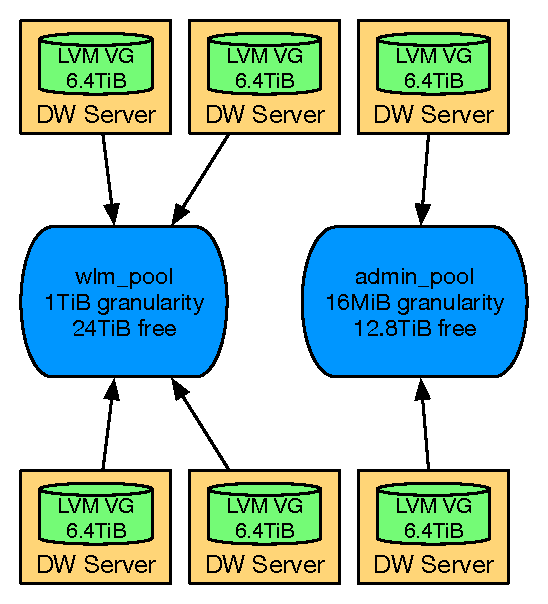
\includegraphics[width=0.8\linewidth]{graphics/node_to_pool}
\caption{Six server nodes belonging to two DataWarp storage pools.  The pool \emph{wlm\_pool} has four nodes worth of storage in it, and instance fragments are created that are multiples of 1TiB.  The pool \emph{admin\_pool} has two nodes worth of storage in it, and instance fragments are created that are multiples of 16MiB.  The larger allocation granularity associated with \emph{wlm\_pool} means that 0.4TiB of space per server node is inaccessible.\label{node_to_pool}}
\end{figure}

The DataWarp service provides instance- and application-based I/O accounting and configurable I/O limits.  Accounting data is collected using RUR~\cite{barry2013resource} and includes statistics such as reads/writes performed per compute node and per server node.

To prevent a runaway application from consuming too much of the remaining device endurance, excess I/O activity detection is determined using three different user- and site-configurable policies:
\begin{itemize}
\item \textbf{Maximum Files Created:} Users that know how many files their application will create can specify an upper bound to DataWarp and have subsequent creates fail.
\item \textbf{Maximum File Size:}  Users that know the maximum file size to ever be read or written by their application can specify an upper bound to have reads and writes in violation of the policy fail.
\item \textbf{Maximum Writes Over Time:} Users that know how much data their application will write over a period of time (e.g., entire batch job, every 2 hours, etc.) can specify a time window and a byte value to establish an upper bound on writes in a rolling window that, when exceeded, will prevent future writes from succeeding.  As time progresses, the window slides forward and writes that occurred outside of the window are no longer counted against the byte threshold.
\end{itemize}

\subsection{Resiliency}
If a DataWarp server node fails, only jobs using instances on the failed node are affected.  Those jobs will see I/O errors. New instance creation requests will avoid failed server nodes.  The WLM will reduce available capacity by that of the failed nodes.

DataWarp periodically monitors the remaining SSD endurance and will stop assigning a server node to new instances when the remaining endurance falls below a configurable threshold. DataWarp server nodes can be drained for maintenance, in which case they do not get assigned new instances and existing job instances are allowed to complete normally.  SSDs can also move to new DataWarp server nodes and existing persistent instances on those SSDs will still be usable by future batch jobs.

DataWarp does not provide any data redundancy. While it would be possible to replicate data across multiple DataWarp servers, the increased HSN and SSD traffic would cause a significant reduction in the effective DataWarp bandwidth (and to a lesser extent, a reduction in capacity and endurance), reducing the cost effectiveness of DataWarp.

\section{Performance}
DataWarp bandwidth is proportional to the number of DataWarp servers used for the instance.  See \figurename~\ref{max_seq_read_rate} for the maximum sequential read rate for a scratch instance when using 1 or 2 DataWarp server nodes vs. Lustre OSTs on Sonexion 2000.  We performed measurements on Cray-owned XC systems running CLE 5.2.UP04 with Phase~1 software.  We used the IOR benchmark running in POSIX file per process mode accessing 192GiB of data.  The DataWarp experiment used 2 ranks per node on 8 or 16 compute nodes for the 1 or 2 servers, respectively.  The Lustre experiment used 2 ranks per node on 16 compute nodes.  Performance suffers at small transfer sizes due to the lack of client-side caching in Phase~1, but exceeds Lustre performance for 64-128KiB and larger transfer sizes.  See \figurename~\ref{max_seq_write_rate} for the maximum sequential write rate for the same setup.  For DataWarp, read and write performance peaks at 512KiB transfer size before decreasing and leveling off.  At 512KiB, the transfer size is large enough to make good use of the Aries network and amortize the fixed RPC cost overhead while being small enough to perform well when the server is low on free memory.

\begin{figure*}
\subfloat[Read]{
\begin{tikzpicture}[baseline]
	\begin{semilogxaxis}[
		xlabel=Transfer Size (bytes),
		ylabel=MB/sec,
		scaled ticks=false,
		grid=major,
		log basis x=2,
		legend style={
			font=\small,
			cells={anchor=west},
			legend pos=north west,
		},
%		xticklabel style={
%      rotate=90,
%      anchor=east,
%      /pgf/number format/fixed,
%},
]
	% 1 node write datawarp
	\addlegendentry{DW 1 node}
	\addplot table {data/max_seq_read_rate_1_dw.csv};
	
	% 2 node write datawarp
	\addlegendentry{DW 2 nodes}
	\addplot table {data/max_seq_read_rate_2_dw.csv};
	
	% 1 node read sonexion 2000
	\addlegendentry{Son. 1 OST}
	\addplot table {data/max_seq_read_rate_1_son.csv};
	
	% 2 node read sonexion 2000
	\addlegendentry{Son. 2 OSTs}
	\addplot table {data/max_seq_read_rate_2_son.csv};

	\end{semilogxaxis}
\end{tikzpicture}
\label{max_seq_read_rate}}
\hfil
\subfloat[Write]{
\begin{tikzpicture}[baseline]
	\begin{semilogxaxis}[
		xlabel=Transfer Size (bytes),
		ylabel=MB/sec,
		scaled ticks=false,
		grid=major,
		ymax = 18750,
		log basis x={2},
		legend style={
			font=\small,
			cells={anchor=west},
			legend pos=north west,
		},
%		xticklabel style={
%      rotate=90,
%      anchor=east,
%      /pgf/number format/fixed,
%},
]
	% 1 node write datawarp
	\addlegendentry{DW 1 node}
	\addplot table {data/max_seq_write_rate_1_dw.csv};
	
	% 2 node write datawarp
	\addlegendentry{DW 2 nodes}
	\addplot table {data/max_seq_write_rate_2_dw.csv};
	
	% 1 node write sonexion 2000
	\addlegendentry{Son. 1 OST}
	\addplot table {data/max_seq_write_rate_1_son.csv};
	
	% 2 node write sonexion 2000
	\addlegendentry{Son. 2 OSTs}
	\addplot table {data/max_seq_write_rate_2_son.csv};
	
	\end{semilogxaxis}
\end{tikzpicture}
\label{max_seq_write_rate}}
\caption{Maximum sequential read rate~(\ref{max_seq_read_rate}) and write rate~(\ref{max_seq_write_rate}) between DataWarp and Sonexion 2000 with one or two servers or OSTs, respectively.}
\end{figure*}

A single compute node can saturate an entire DataWarp server node for both reads and writes if enough streams are used.  See \figurename~\ref{max_seq_read_rate_single_compute} for reads and \figurename~\ref{max_seq_write_rate_single_compute} for writes.  For reads, saturation occurs at around 8 streams per node.  For writes, saturation occurs at around 16 streams per node.

\begin{figure*}
\subfloat[Read]{
\begin{tikzpicture}[baseline]
	\begin{semilogxaxis}[
		xlabel=Transfer Size (bytes),
		ylabel=MB/sec,
		scaled ticks=false,
		grid=major,
		log basis x=2,
		legend style={
			font=\small,
			cells={anchor=west},
			legend pos=north west,
		},
%		xticklabel style={
%      rotate=90,
%      anchor=east,
%      /pgf/number format/fixed,
%},
]
	% 1 file
	\addlegendentry{1 file}
	\addplot table {data/max_seq_read_rate_dw_1_file.csv};
	
	% 2 files
	\addlegendentry{2 files}
	\addplot table {data/max_seq_read_rate_dw_2_files.csv};
	
	% 4 files
	\addlegendentry{4 files}
	\addplot table {data/max_seq_read_rate_dw_4_files.csv};
		
	% 8 files
	\addlegendentry{8 files}
	\addplot table {data/max_seq_read_rate_dw_8_files.csv};
	
	% 16 files
	\addlegendentry{16 files}
	\addplot table {data/max_seq_read_rate_dw_16_files.csv};
	
	% 32 files
	\addlegendentry{32 files}
	\addplot table {data/max_seq_read_rate_dw_32_files.csv};
	
	\end{semilogxaxis}
\end{tikzpicture}
\label{max_seq_read_rate_single_compute}}
\hfil
\subfloat[Write]{
\begin{tikzpicture}[baseline]
	\begin{semilogxaxis}[
		xlabel=Transfer Size (bytes),
		ylabel=MB/sec,
		scaled ticks=false,
		grid=major,
		log basis x=2,
		ymax=8800,
		legend style={
			font=\small,
			cells={anchor=west},
			legend pos=north west,
		},
%		xticklabel style={
%      rotate=90,
%      anchor=east,
%      /pgf/number format/fixed,
%},
]
	% 1 file
	\addlegendentry{1 file}
	\addplot table {data/max_seq_write_rate_dw_1_file.csv};
	
	% 2 files
	\addlegendentry{2 files}
	\addplot table {data/max_seq_write_rate_dw_2_files.csv};
	
	% 4 files
	\addlegendentry{4 files}
	\addplot table {data/max_seq_write_rate_dw_4_files.csv};
		
	% 8 files
	\addlegendentry{8 files}
	\addplot table {data/max_seq_write_rate_dw_8_files.csv};
	
	% 16 files
	\addlegendentry{16 files}
	\addplot table {data/max_seq_write_rate_dw_16_files.csv};
	
	% 32 files
	\addlegendentry{32 files}
	\addplot table {data/max_seq_write_rate_dw_32_files.csv};
	
	\end{semilogxaxis}
\end{tikzpicture}
\label{max_seq_write_rate_single_compute}}
\caption{Maximum sequential read rate~(\ref{max_seq_read_rate_single_compute}) and write rate~(\ref{max_seq_write_rate_single_compute}) from one compute node to one DataWarp server node for varying numbers of file streams.}
\end{figure*}

The MSC Nastran structural analysis software~\cite{nastran} exhibits an I/O pattern on some data files that is challenging for spinning disk hardware.  Data files are repeatedly read sequentially both forward and backward.  On forward passes, prefetching enables fast performance.  On backward passes, prefetching is bypassed and the storage hardware must be involved with every read operation.  DataWarp's SSD hardware allows for these reads to complete without access penalty, whereas PFS spinning disk hardware must frequently perform expensive seeks.  \figurename~\ref{nastran} shows a comparison using MSC Nastran between a DataWarp environment and a Lustre environment.  This example displays file position over time accessing the SCR300 file, showing the forward and backward passes of reading the factored matrix.  DataWarp performance in the forward and backward passes is consistent and fast.  On sequential backwards reads, Lustre performance performs well at first due to cache hits in the client cache from spatial locality, but suffers once the spinning disk hardware is accessed.  The end result is the DataWarp environment performs twice as fast.

%\begin{figure*}
%\centering
%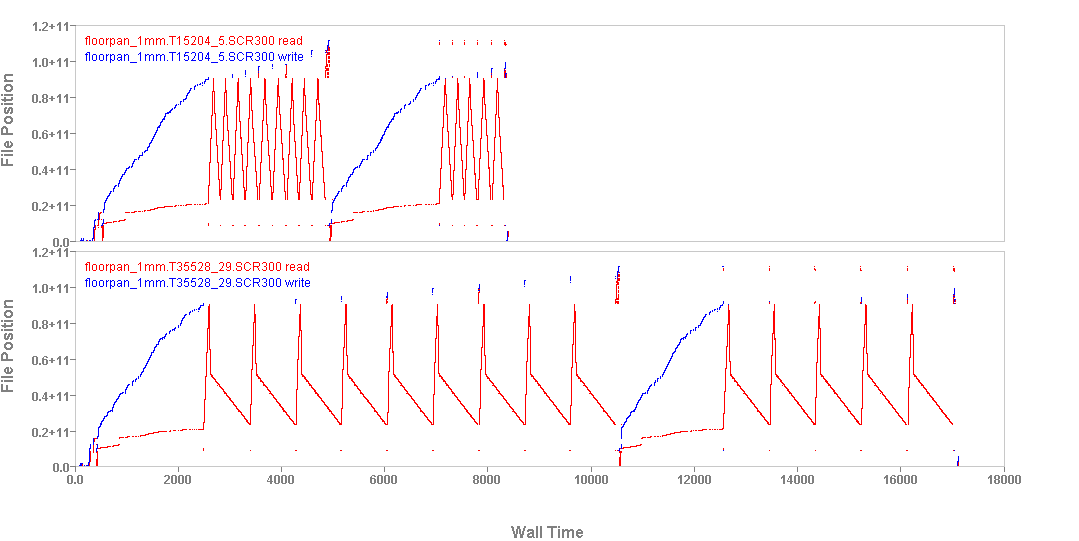
\includegraphics[width=\textwidth]{graphics/nastran_tmp}
%\caption{NASTRAN performs sequential reads forwards and backwards multiple times.  Traditional spinning disks suffer while reading sequentially backwards due to expensive seeks while DataWarp SSD hardware does not suffer the same penalty.  Image generated with IOT toolkit from I/O Doctors, LLC and used with permission.\label{nastran}}
%\end{figure*}
\begin{figure*}
\centering
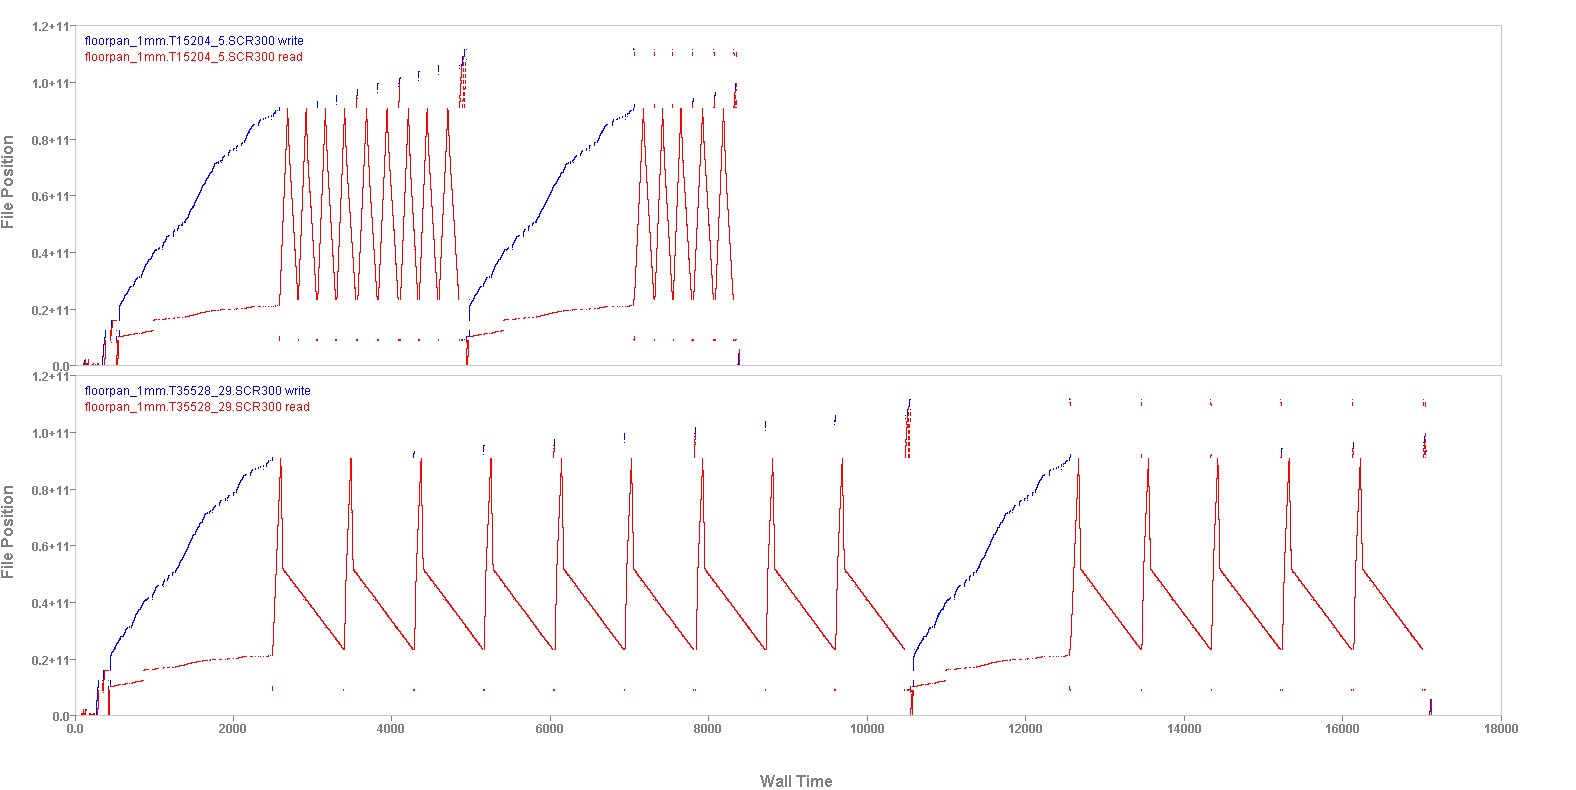
\includegraphics[width=\textwidth]{graphics/predat_FPA_1576x790}
\caption{NASTRAN performs sequential reads forwards and backwards multiple times.  Traditional spinning disks suffer while reading sequentially backwards due to expensive seeks while DataWarp SSD hardware does not suffer the same penalty.  Image courtesy of I/O Doctors, LLC.\label{nastran}}
\end{figure*}

DataWarp performance scales to larger environments.  \figurename~\ref{kaust} shows the results of running the IOR benchmark on a customer installation with 264 DataWarp servers, each with 2 Intel P3608 SSDs~\cite{intel-p3608}.  The test was IOR POSIX file per process running on 5280 compute nodes, 2 ranks per node, and 10560 ranks running Phase~1 DataWarp on CLE5.2.UP04.  Additional parameters include a transfer size of 512KiB with 16GiB of data per file, and all files striped across all servers.  In aggregate, the write rate achieved 1.54 TB/sec and the read rate achieved 1.66 TB/sec.

%Summary of the IOR results.  ~170 TB of data (32 GiB from each of 5280 nodes):
% 
%        api                = POSIX
%        test filename      = /var/opt/cray/dws/mounts/batch/424171/ss//IOR_file
%        access             = file-per-process
%        pattern            = segmented (1 segment)
%        ordering in a file = sequential offsets
%        ordering inter file=constant task offsets = 1
%        clients            = 10560 (2 per node)
%        repetitions        = 1
%        xfersize           = 524288 bytes
%        blocksize          = 16 GiB
%        aggregate filesize = 168960 GiB
% 
%About 3 million IOPS with 512 KiB transfers.

%\begin{figure}
%\centering
%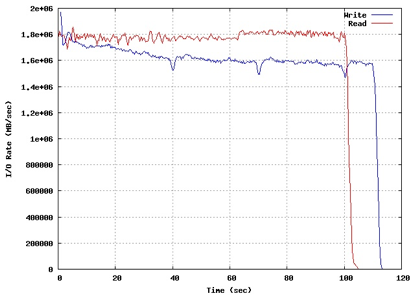
\includegraphics[width=\linewidth]{graphics/kaust_tmp}
%\caption{KAUST example\label{kaust2}}
%\end{figure}

\begin{figure*}
\centering
\begin{tikzpicture}
	\begin{axis}[
		xlabel=Time (seconds),
		ylabel=I/O Rate (MB/sec),
		scaled ticks=false,
		width=0.95\textwidth,
		extra y ticks={1750000},
		height=5cm,
		grid=major,
		xmin=0, ymin=0, xmax=120, ymax=2000000,
%		enlargelimits=false,
		every axis plot post/.append style={mark=none},
		legend style={
			font=\small,
			cells={anchor=west},
			legend pos=south west,
		},
	]
	% Write
	\addlegendentry{Write}
	\addplot table {data/striped_512k_5280nodes_10560files_16g_424171.WriteRate.csv};
	% Read
	\addlegendentry{Read}
	\addplot table {data/striped_512k_5280nodes_10560files_16g_424171.ReadRate.csv};
	\end{axis}
\end{tikzpicture}
\caption{Results from running the IOR benchmark in POSIX file per process mode on 5280 compute nodes with 2 ranks per node against 264 DataWarp servers.\label{kaust}}
\end{figure*}

% An example of a floating figure using the graphicx package.
% Note that \label must occur AFTER (or within) \caption.
% For figures, \caption should occur after the \includegraphics.
% Note that IEEEtran v1.7 and later has special internal code that
% is designed to preserve the operation of \label within \caption
% even when the captionsoff option is in effect. However, because
% of issues like this, it may be the safest practice to put all your
% \label just after \caption rather than within \caption{}.
%
% Reminder: the "draftcls" or "draftclsnofoot", not "draft", class
% option should be used if it is desired that the figures are to be
% displayed while in draft mode.
%
%\begin{figure}[!t]
%\centering
%\includegraphics[width=2.5in]{myfigure}
% where an .eps filename suffix will be assumed under latex, 
% and a .pdf suffix will be assumed for pdflatex; or what has been declared
% via \DeclareGraphicsExtensions.
%\caption{Simulation results for the network.}
%\label{fig_sim}
%\end{figure}

% Note that the IEEE typically puts floats only at the top, even when this
% results in a large percentage of a column being occupied by floats.


% An example of a double column floating figure using two subfigures.
% (The subfig.sty package must be loaded for this to work.)
% The subfigure \label commands are set within each subfloat command,
% and the \label for the overall figure must come after \caption.
% \hfil is used as a separator to get equal spacing.
% Watch out that the combined width of all the subfigures on a 
% line do not exceed the text width or a line break will occur.
%
%\begin{figure*}[!t]
%\centering
%\subfloat[Case I]{\includegraphics[width=2.5in]{box}%
%\label{fig_first_case}}
%\hfil
%\subfloat[Case II]{\includegraphics[width=2.5in]{box}%
%\label{fig_second_case}}
%\caption{Simulation results for the network.}
%\label{fig_sim}
%\end{figure*}
%
% Note that often IEEE papers with subfigures do not employ subfigure
% captions (using the optional argument to \subfloat[]), but instead will
% reference/describe all of them (a), (b), etc., within the main caption.
% Be aware that for subfig.sty to generate the (a), (b), etc., subfigure
% labels, the optional argument to \subfloat must be present. If a
% subcaption is not desired, just leave its contents blank,
% e.g., \subfloat[].


% An example of a floating table. Note that, for IEEE style tables, the
% \caption command should come BEFORE the table and, given that table
% captions serve much like titles, are usually capitalized except for words
% such as a, an, and, as, at, but, by, for, in, nor, of, on, or, the, to
% and up, which are usually not capitalized unless they are the first or
% last word of the caption. Table text will default to \footnotesize as
% the IEEE normally uses this smaller font for tables.
% The \label must come after \caption as always.
%
%\begin{table}[!t]
%% increase table row spacing, adjust to taste
%\renewcommand{\arraystretch}{1.3}
% if using array.sty, it might be a good idea to tweak the value of
% \extrarowheight as needed to properly center the text within the cells
%\caption{An Example of a Table}
%\label{table_example}
%\centering
%% Some packages, such as MDW tools, offer better commands for making tables
%% than the plain LaTeX2e tabular which is used here.
%\begin{tabular}{|c||c|}
%\hline
%One & Two\\
%\hline
%Three & Four\\
%\hline
%\end{tabular}
%\end{table}


% Note that the IEEE does not put floats in the very first column
% - or typically anywhere on the first page for that matter. Also,
% in-text middle ("here") positioning is typically not used, but it
% is allowed and encouraged for Computer Society conferences (but
% not Computer Society journals). Most IEEE journals/conferences use
% top floats exclusively. 
% Note that, LaTeX2e, unlike IEEE journals/conferences, places
% footnotes above bottom floats. This can be corrected via the
% \fnbelowfloat command of the stfloats package.




\section{Conclusion}
Provisioning a PFS for both bandwidth and capacity on large HPC systems is cost-prohibitive.  DataWarp introduces a storage layer between user applications and the PFS to handle the application's bandwidth needs, which allows the PFS to be provisioned primarily for capacity and resiliency requirements.  Interaction between DataWarp and the PFS can happen asynchronously to applications, which reduces the quantity of time that compute nodes need to be allocated to jobs while allowing them to spend more time being used for computation.  DataWarp instances can be created on demand per batch job, or they can be shared amongst multiple batch jobs in order to further minimize PFS interaction.

DataWarp accelerates many use cases.  As a PFS cache, it accelerates applications that perform checkpoint/restart, have periodic output, or use lots of application library files.  As a \texttt{/tmp} replacement, it allows for applications to dump state without ever performing PFS I/O or consuming valuable compute node memory.  Users can use persistent instances to access frequently used shared data files or have multiple jobs manipulate data before eventually writing final results to a PFS.  Using DataWarp for swap files on compute nodes enables applications needing more memory than is present on those nodes to complete successfully.  If applications are run directly on DataWarp server nodes they have access to the high IOPS rate provided by the SSD hardware.

DataWarp is capable of providing superior bandwidth compared to a traditional PFS due to the use of high-performance SSDs and a shorter path between compute nodes and DataWarp servers.  A single compute node is capable of saturating a single DataWarp server node, and DataWarp scales to hundreds of servers.




% conference papers do not normally have an appendix



% use section* for acknowledgment
\ifCLASSOPTIONcompsoc
  % The Computer Society usually uses the plural form
  \section*{Acknowledgments}
\else
  % regular IEEE prefers the singular form
  \section*{Acknowledgment}
\fi

The authors would like to thank their teams and users at Cray, LANL, NERSC, and KAUST as well as those working in support of DataWarp at Adaptive, Altair, and SchedMD.





% trigger a \newpage just before the given reference
% number - used to balance the columns on the last page
% adjust value as needed - may need to be readjusted if
% the document is modified later
%\IEEEtriggeratref{8}
% The "triggered" command can be changed if desired:
%\IEEEtriggercmd{\enlargethispage{-5in}}

% references section

% can use a bibliography generated by BibTeX as a .bbl file
% BibTeX documentation can be easily obtained at:
% http://mirror.ctan.org/biblio/bibtex/contrib/doc/
% The IEEEtran BibTeX style support page is at:
% http://www.michaelshell.org/tex/ieeetran/bibtex/
\bibliographystyle{IEEEtran}
% argument is your BibTeX string definitions and bibliography database(s)
\bibliography{IEEEabrv,sources}
%
% <OR> manually copy in the resultant .bbl file
% set second argument of \begin to the number of references
% (used to reserve space for the reference number labels box)

% that's all folks
\end{document}


